\documentclass[xcolor={dvipsnames}]{beamer}
\mode<presentation>
{
  \usetheme{default}
  \usecolortheme{default}
  \usefonttheme{default}
  \setbeamertemplate{navigation symbols}{}
  \setbeamertemplate{caption}[numbered]
} 

\usepackage[english]{babel}
\usepackage[utf8x]{inputenc}
\usepackage[T1]{fontenc}
\usepackage{pdfpages}
\usepackage{changepage}
\usepackage{standalone}
\usepackage[outline]{contour}
\usepackage{graphicx}
\usepackage[geometry]{ifsym} % shape-code the groups
\usepackage{hyperref}
\usepackage{tikz}
\usepackage{tabularx}
\usetikzlibrary{fit}
\usepackage{tipa}
\usepackage{natbib}
\usepackage{forest}
\usepackage{amsmath}
\usepackage{mathtools} 
\usepackage{fontawesome}
\usepackage{transparent}
\usepackage{dsfont} % real numbers symbol
\usetikzlibrary{decorations.pathreplacing}

\title{Clustering Dialect Varieties Based on Historical Sound Correspondences}
\author{Verena Blaschke}
\date{October 10th, 2019\\GSCL Student Talks}
\addtobeamertemplate{title page}{}{\footnotesize\begin{center}Bachelor's Thesis\\Supervised by Dr. Çağrı Çöltekin\\Eberhard Karls Universität Tübingen\end{center}}

% For the map keys.
\definecolor{purple}{HTML}{520066}
\definecolor{midblue}{HTML}{31688e}
\definecolor{green}{HTML}{35b779}
\def\upper{\color{purple}\FilledBigTriangleUp}
\def\central{\color{midblue}\FilledBigSquare}
\def\dutch{\color{green}\FilledBigCircle}
\def\ingv{\color{green}\BigCircle}

% For specifying matrix dimensions. (set of real numbers symbol)
\newcommand{\R}{\mathds{R}}

\newcommand{\hugeSymbol}[1]{{\fontsize{35}{42}\selectfont #1}}

% https://tex.stackexchange.com/questions/331691/how-can-i-get-a-matrix-with-row-and-column-labels-that-can-also-be-aligned-with
\newcommand{\indsize}{\scriptsize}
\newcommand{\colind}[2]{\displaystyle\smash{\mathop{#1}^{\raisebox{.5\normalbaselineskip}{\indsize #2}}}}
\newcommand{\rowind}[1]{\mbox{\indsize #1}}

\begin{document}
\begin{frame}
  \titlepage
\end{frame}
% As the title suggests: my thesis involves both closely related language varieties and historical linguistics


\begin{frame}{Introduction}
Historical linguistics \& dialectology

\vspace{2em}

\hspace{0.15\textwidth}\hugeSymbol{\faBook}\hspace{0.15\textwidth}\hugeSymbol{\faArrowsH}\hspace{0.15\textwidth}\hugeSymbol{\faLaptop}

\vspace{1em}

\begin{itemize}
    \item Efficiency / amount of data vs. time
    \item Feature selection
\end{itemize}
\end{frame}
% Research in historical linguistics and dialectology has traditionally been carried out manually, but in the past decade, computational methods have gained popularity too. The big advantage of using computers: we can quickly analyze data from a lot of language varieties at the same time. The way we pick types of features is still based on previous, manual research. But we can quantitatively determine *which* features are relevant.
% Features: here on a phonetic level, namely based on regular sound correspondences -- I'll get back to that in a minute

\begin{frame}{Introduction}
My BA thesis:
\vspace{1em}
\begin{itemize}
    \item Modern continental West Germanic dialects
    \item Regular sound changes from Proto-Germanic\\(historical linguistics angle!)
    \vspace{1em}
    \item Can we meaningfully cluster the dialects based on shared sound changes?
    \item Compare two clustering methods
\end{itemize}
\end{frame}
% So what did I do?
% CWG: associated with German, Dutch, Frisian
% Proto-Germanic: there exists similar research on clustering dialects, but based on only modern dialects, without the historical linguistics angle
% change = regular sound changes
% traditional research? controversies!
% two clustering methods, two sets of features

\begin{frame}{Data}
\begin{minipage}{.6\textwidth}
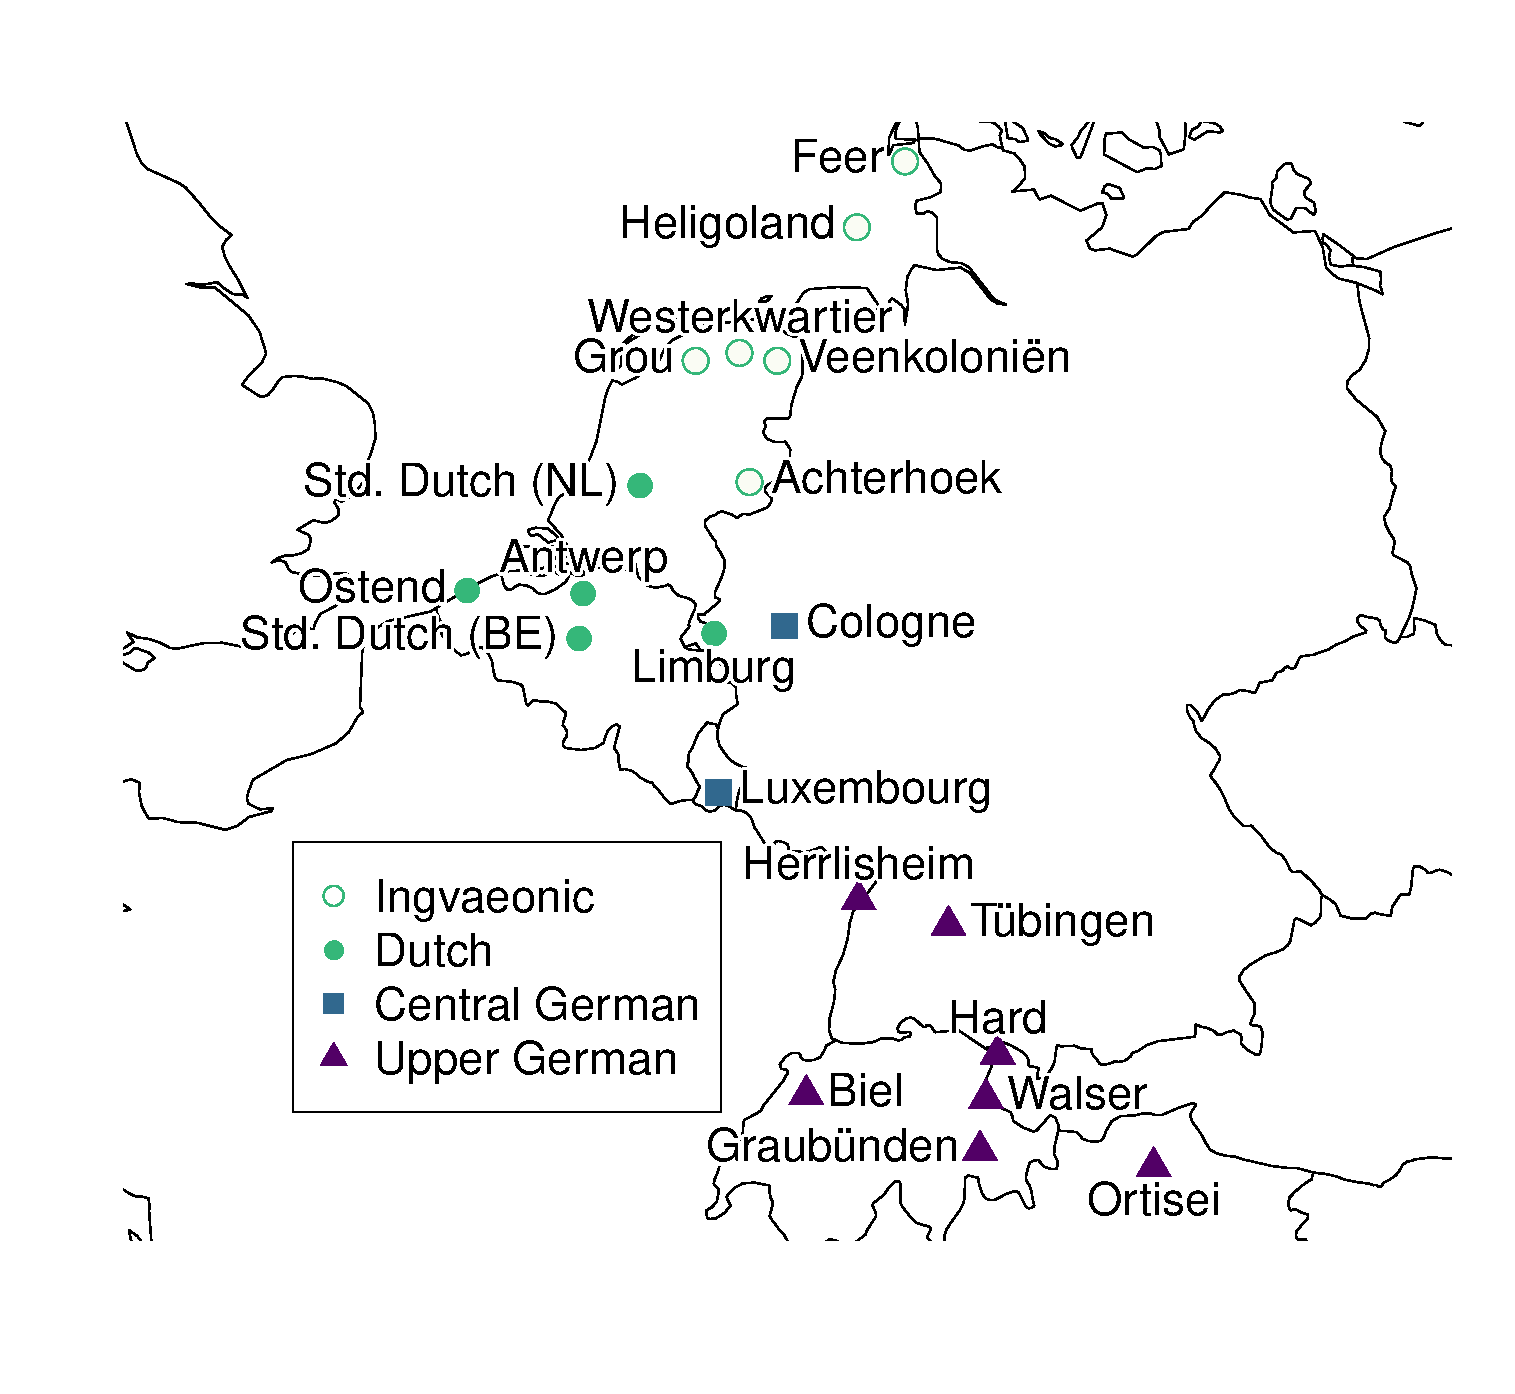
\includegraphics[width=\textwidth,trim={4cm 0 5cm 0},clip]{figures/map-pres.pdf}
\end{minipage}%
\begin{minipage}{.4\textwidth}
Sound Comparisons\\(Heggarty, 2018)
\begin{itemize}
    \item 20 modern dialects
    \item Reconstruction of Proto-Germanic
    \item 110 cognate sets
\end{itemize}
\end{minipage}
\end{frame}

\begin{frame}{Data}{A Gold Standard?}
\vspace{-1.1em}
\begin{minipage}{.6\textwidth}
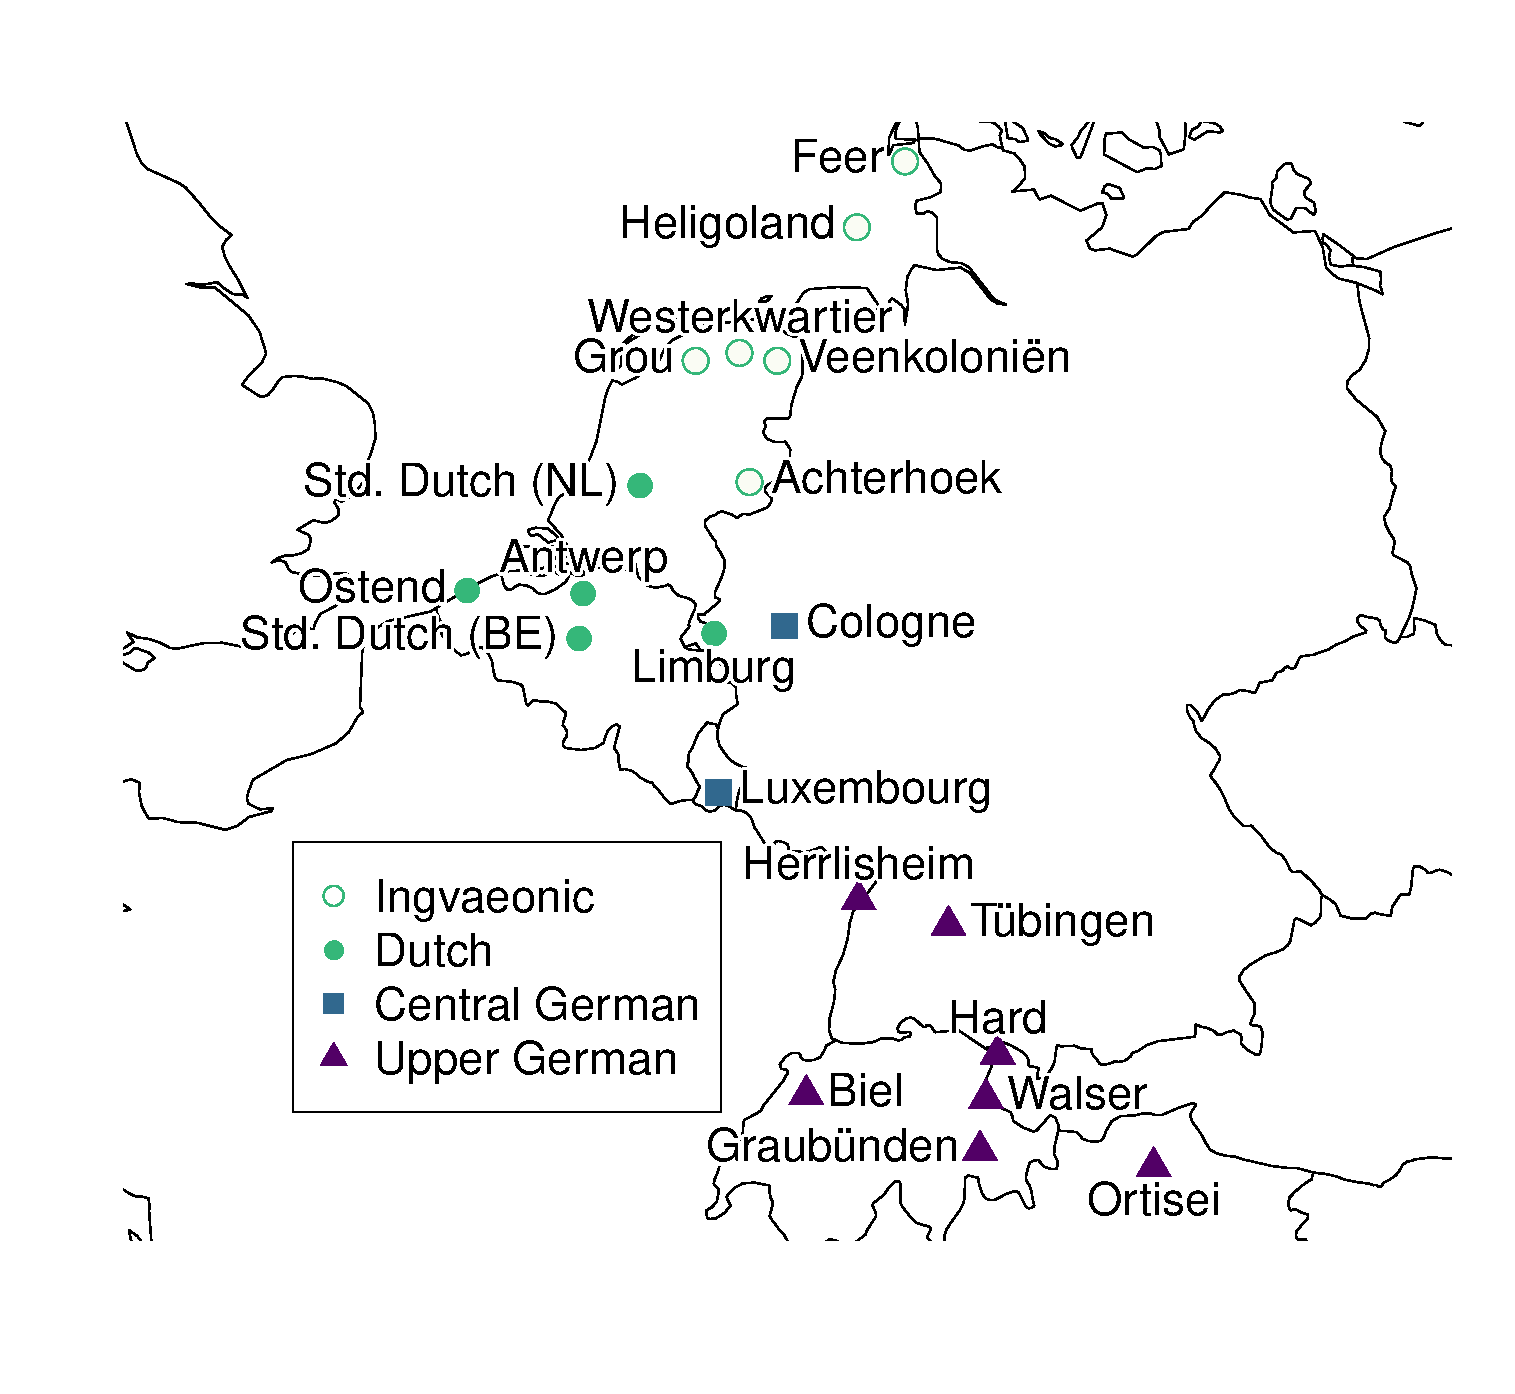
\includegraphics[width=\textwidth,trim={4cm 0 5cm 0},clip]{figures/map-pres.pdf}
\end{minipage}%
\begin{minipage}{.41\textwidth}
\begin{itemize}
    \item Ingv\ae{}onic (North Sea Germanic) vs. rest
    \pause
    \item High German sound shift\\
    \begin{itemize}
        \item /*p/ $>$ /\texttoptiebar{pf}/ or /f/
        \item /*t/ $>$ /\texttoptiebar{ts}/ or /s/
        \item /*k/ $>$ /\texttoptiebar{kx}/ or /x/
        % \item /*b,~*d,~*g/ $>$ /*p,~*t,~*k/
    \end{itemize}
    (Upper, Central, Low DE + NL/Fris)
    % \pause
    % \item Splits vs. waves
\end{itemize}
\end{minipage}
\end{frame}
% v similar dialects, but there exist some common ways of grouping them
% Ingv: difficult to define; mostly based on inflections and pronouns, here: Frisian (and Low German), although some would also include Dutch (next split)
% sound shift: most characteristically: lenition of voiceless stops. depends on position within a word, the word itself, and the sound; transition zones, no hard boundary between low and central German. there are no low German dialects in the data I worked with, but otherwise they would have been included in the Ingv group. central and upper German in opposition to low German, Dutch and Frisian
% controversy around continental West Germanic: historical changes (splits) vs. mutual influences (wave-like), tree-like vs. dialect continuum

\begin{frame}[t]{Method}{}
{\usebeamercolor[fg]{structure} 1.} Align segments \hspace{0.5em} {\usebeamercolor[fg]{structure} 2.} Deduce sound changes \hspace{0.5em} {\usebeamercolor[fg]{structure} 3.} Cluster dialects
\end{frame}

\newcounter{nodecount}
\newcommand\tabnode[1]{\addtocounter{nodecount}{1} \tikz \node  (\arabic{nodecount}) {#1};}

\begin{frame}[t]{Method}{}
{\usebeamercolor[fg]{structure} 1.} Align segments \hspace{0.5em} {\transparent{0.4} {\usebeamercolor[fg]{structure} 2.} Deduce sound changes \hspace{0.5em} {\usebeamercolor[fg]{structure} 3.} Cluster dialects}

\vspace{2em}
\includestandalone[]{tables/msa-pres}

\vspace{1em}
Progressive multiple sequence alignment\\(Notredame et al., 2000)
\end{frame}


\begin{frame}[t]{Method}{}
{\transparent{0.4} {\usebeamercolor[fg]{structure} 1.} Align segments} \hspace{0.5em} {\usebeamercolor[fg]{structure} 2.} Deduce sound changes \hspace{0.5em} {\transparent{0.4} {\usebeamercolor[fg]{structure} 3.} Cluster dialects}

\vspace{2em}
\includestandalone[]{tables/msa-pres-red}

\pause
\vspace{1em}
\begin{tabular}{ll}
k $>$ x & no context \\
k $>$ x / \# \_ & word boundaries \\
k $>$ x / \_ vow &  simple context (cons/vow)\\
k $>$ x / \_ A & sound class-based context (List, 2012)
\end{tabular}
\end{frame}
% direct left-hand and right-hand context
% context only when it is identical
% sound classes: 15 consonant groups, six vowel groups
% ignore rare sound correspondences (probably not regular), less than three occurrences
% unrounded open vowels

\begin{frame}[t]{Method}{}
{\transparent{0.4} {\usebeamercolor[fg]{structure} 1.} Align segments} \hspace{0.5em} {\usebeamercolor[fg]{structure} 2.} Deduce sound changes \hspace{0.5em} {\transparent{0.4} {\usebeamercolor[fg]{structure} 3.} Cluster dialects}

\vspace{2em}
\includestandalone[]{tables/msa-pres-red}

\vspace{1em}
\begin{minipage}{0.3\textwidth}
\begin{tabular}{l}
k $>$ x\\
k $>$ x / \# \_\\
k $>$ x / \_ vow\\
k $>$ x / \_ A
\end{tabular}
\end{minipage}%
\begin{minipage}{0.7\textwidth}

% \vspace{1em}
\[
  \begin{array}{@{}c@{}}
    \rowind{Walser} \\ \rowind{Biel} \\ \rowind{Lux.} \\ \rowind{Westk.} \\ \rowind{...}
  \end{array}
  \mathop{\left[
  \begin{array}{ *{3}{c} }
     \colind{1}{k $>$ x}  &  \colind{1}{k $>$ x / \#\_}  &  \colind{...}{...} \\
    0 &  0  &  ... \\
     0  & 0 &  ... \\
     0  &  0  & ... \\
     ...  &  ...  &  ...
  \end{array}
  \right]}
\]
\end{minipage}
\end{frame}
% dialect-by-sound-correspondence frequency matrix

\begin{frame}[t]{Method}{}
{\transparent{0.4} {\usebeamercolor[fg]{structure} 1.} Align segments \hspace{0.5em} {\usebeamercolor[fg]{structure} 2.} Deduce sound changes} \hspace{0.5em} {\usebeamercolor[fg]{structure} 3.} Cluster dialects

\vspace{2em}
\begin{itemize}
    \item Clustering only dialects vs. clustering dialects and sound correspondences at the same time
    \item Sound correspondences without/with phonetic context
\end{itemize}

\pause
\vspace{2em}
Both clustering methods:
\begin{enumerate}
    \item Normalize the dialect-by-correspondence tally matrix
    \item Hierarchical clustering
\end{enumerate}
\end{frame}
% Cluster only dialects: infer relevant sound changes afterwards
% Normalization: adjust feature frequencies by how informative they are

\begin{frame}[t]{Method}{}
{\transparent{0.4} {\usebeamercolor[fg]{structure} 1.} Align segments \hspace{0.5em} {\usebeamercolor[fg]{structure} 2.} Deduce sound changes} \hspace{0.5em} {\usebeamercolor[fg]{structure} 3.} Cluster dialects

\vspace{2em}
Clustering only dialects (agglomerative clustering)
\begin{enumerate}
    \item Normalization: TF-IDF weighting
    \item Clustering:
    Dialect-by-correspondence matrix \faArrowRight{} dialect-by-dialect distance matrix
        \faArrowRight{} dendrogram
\end{enumerate}

\pause
\vspace{2em}
Clustering dialects and sound correspondences (bipartite spectral graph co-clustering (Dhillon, 2001; Wieling and Nerbonne, 2010))

\begin{enumerate}
    \item Normalization: Map all dialects and sound correspondences to vectors in a shared vector space
    \item Clustering: K-means clustering (k=2)
    \item Repeat
\end{enumerate}
\end{frame}
% cluster dialects, infer relevant sound correspondences later
% cosine distance
% cluster dialects and sound correspondences at the same time
% keep repeating both steps

\begin{frame}[t]{Method}{}
{\transparent{0.4} {\usebeamercolor[fg]{structure} 1.} Align segments \hspace{0.5em} {\usebeamercolor[fg]{structure} 2.} Deduce sound changes} \hspace{0.5em} {\usebeamercolor[fg]{structure} 3.} Cluster dialects

\vspace{4em}
\begin{itemize}
    \item  Now we have clusters of dialects / dialects and sound correspondences
    \item Rank the sound correspondences in each cluster: 
        \begin{itemize}
        \item Representativeness
        \item Distinctiveness
        \item Frequency
        \end{itemize}
\end{itemize}
\end{frame}
% Tree structure that we can cut to obtain clusters
% representativeness: What proportion of dialects in a given cluster exhibit a given sound correspondence? 
% distinctiveness: How often does a given sound correspondence occur in a given cluster compared to other clusters?
% harmonic mean

\begin{frame}{Results \& Discussion}
No context vs. context
\begin{itemize}
    \item With context: Higher representativeness \& distinctiveness scores
    \item High-ranking sound correspondences often with consonant/vowel or word boundary information
\end{itemize}

\pause
Clustering methods
\begin{itemize}
    \item Agglomerative clustering: More high-ranking sound correspondences, closer to the literature
    \item Graph co-clustering: Worked well in other researchers' dialectometry experiments -- effects of data selection and pre-processing
\end{itemize}
\end{frame}
% No context vs. context: regardless of clustering method. context: balance for generalizing to the data
% Aggl vs graph: regardless of context granularity

\begin{frame}{}
\hspace{-2.9em}\vspace{-1.3em}\begin{tikzpicture}
    \node[anchor=south west,inner sep=0] (image) at (0,0) {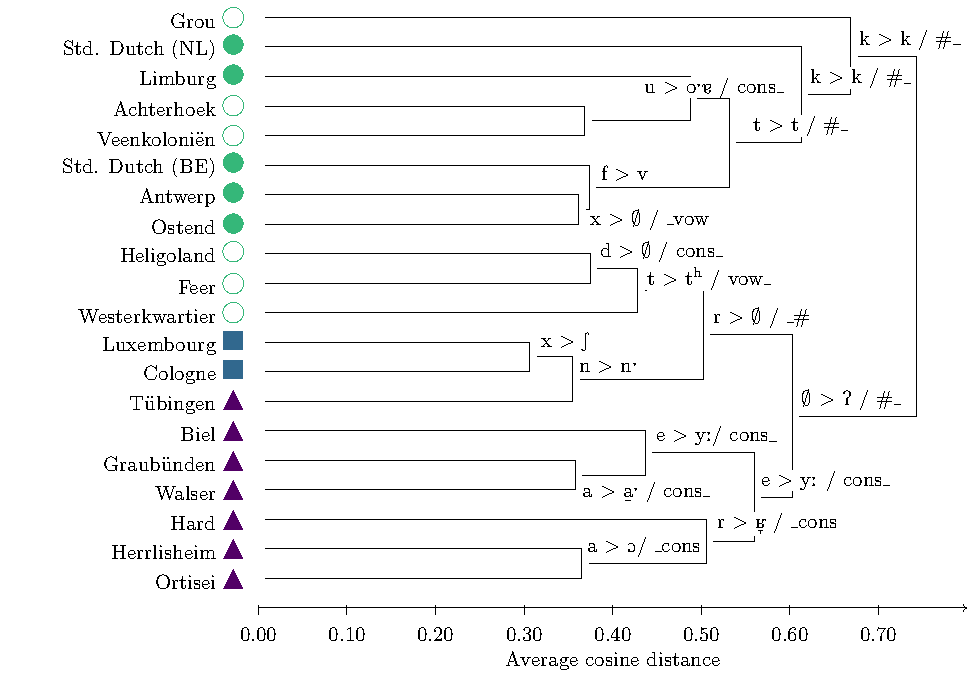
\includegraphics[width=1.1\textwidth]{figures/tfidf-context.pdf}};
\end{tikzpicture}
\vspace{-1em}
\begin{center}
\small
{\ingv} Ingv\ae{}onic \hspace{1em}
{\dutch} Dutch \hspace{1em}
{\central} Central German \hspace{1em}
{\upper} Upper German
\end{center}
\end{frame}
% "Best" result: agglomerative clustering with phonetic context
% dendrogram visualizing which dialects are clustered together how closely, plus highest-ranking sound change per cluster

% https://tex.stackexchange.com/questions/9559/drawing-on-an-image-with-tikz/9562
\begin{frame}{}
\hspace{-2.9em}\vspace{-1.3em}\begin{tikzpicture}
    \node[anchor=south west,inner sep=0] (image) at (0,0) {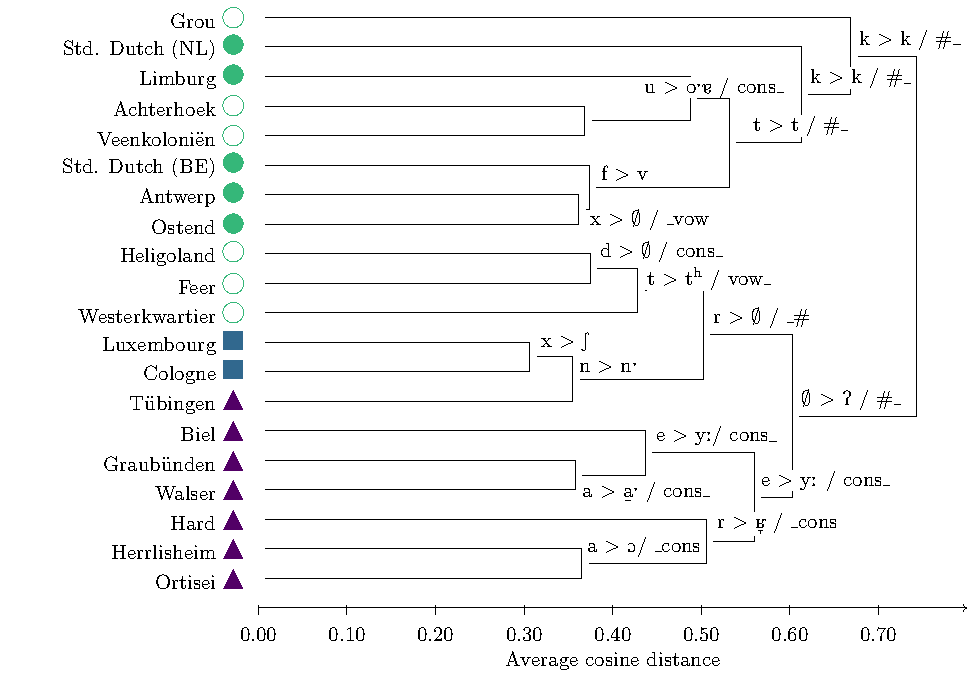
\includegraphics[width=1.1\textwidth]{figures/tfidf-context.pdf}};
   \begin{scope}[x={(image.south east)},y={(image.north west)}]
        \draw[red,ultra thick,rounded corners] (0.05,0.95) rectangle (0.27,0.999);
        \draw[red,ultra thick,rounded corners] (0.05,0.77) rectangle (0.27,0.87);
        \draw[red,ultra thick,rounded corners] (0.05,0.51) rectangle (0.27,0.65);
    \end{scope}
\end{tikzpicture}
\vspace{-1em}
\begin{center}
\small
{\ingv} Ingv\ae{}onic \hspace{1em}
{\dutch} Dutch \hspace{1em}
{\central} Central German \hspace{1em}
{\upper} Upper German
\end{center}
\end{frame}
% Ingvaeonic: (at best) mixed with Dutch and Central German dialects -- see controversy around definition
% posited phonological characteristics not reflected

\begin{frame}{}
\hspace{-2.9em}\vspace{-1.3em}\begin{tikzpicture}
    \node[anchor=south west,inner sep=0] (image) at (0,0) {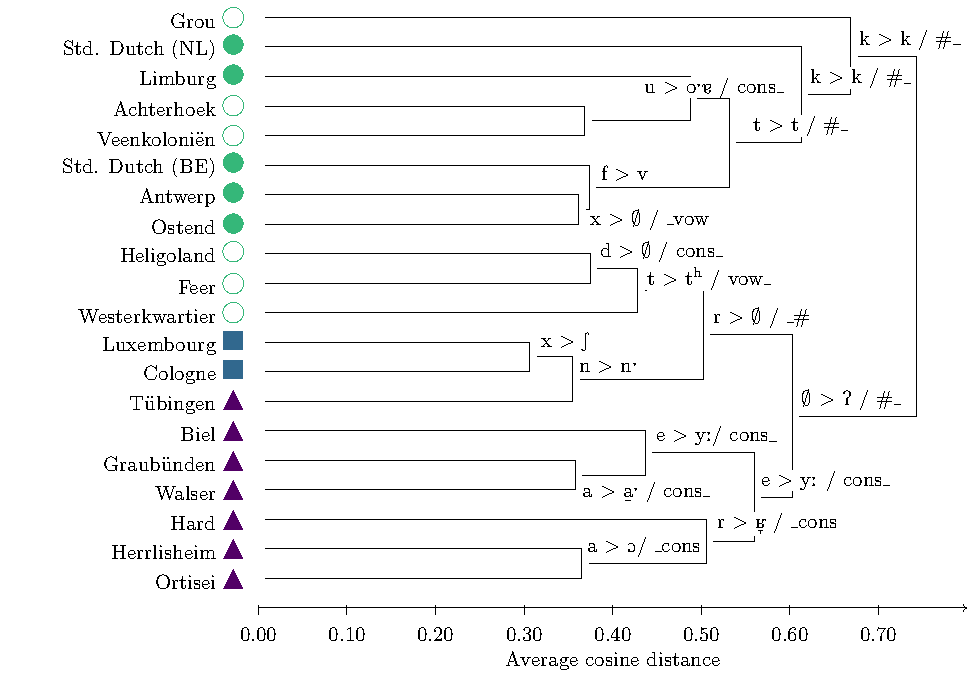
\includegraphics[width=1.1\textwidth]{figures/tfidf-context.pdf}};
   \begin{scope}[x={(image.south east)},y={(image.north west)}]
        \draw[red,ultra thick,rounded corners] (0.05,0.38) rectangle (0.27,0.52);
        \draw[red,ultra thick,rounded corners] (0.05,0.12) rectangle (0.27,0.38);
        \draw[red,ultra thick,rounded corners] (0.75,0.77) rectangle (0.999,0.99);
    \end{scope}
\end{tikzpicture}
\vspace{-1em}
\begin{center}
\small
{\ingv} Ingv\ae{}onic \hspace{1em}
{\dutch} Dutch \hspace{1em}
{\central} Central German \hspace{1em}
{\upper} Upper German
\end{center}
\end{frame}
% High German sound shift:
% (agglomerative + context): reflected in clusters and sound correspondences
% Dutch and Ingvaeonic: preservation of Proto-Germanic voiceless stops


\begin{frame}{Results}
\begin{figure}[h]
\begin{adjustwidth}{-2cm}{-2cm}
\centering
\includestandalone[width=0.65\textwidth]{figures/cosine}
\pause
\hspace{-7em}
\includestandalone[width=0.65\textwidth]{figures/cosine2}
\end{adjustwidth}
\end{figure}
\end{frame}
% distance matrix the agglomerative clustering approach is
% Splits and/or waves?
% Not only clusters, but also a net-like connection between all dialects!
% try out fuzzy clustering?

\begin{frame}{Conclusion}
\begin{itemize}
    \item We can infer meaningful structures
    \item Phonetic context is important!
    \item The simple approach (clustering only dialects) does better
\end{itemize}

\vspace{2em}
\url{github.com/verenablaschke/dialect-clustering}
\end{frame}
% open questions

\appendix
\begin{frame}[allowframebreaks]{Bibliography}
\begin{itemize}
    \item 
Dhillon, I. S. (2001). Co-clustering Documents and Words Using Bipartite Spectral Graph Partitioning.\\
In \textit{Proceedings of the Seventh ACM SIGKDD International Conference on Knowledge
Discovery and Data Mining}, KDD ’01, San Francisco, pp. 269–274. ACM.

\item
Heggarty, P. (2018). Sound Comparisons: Exploring Diversity in Phonetics across Language
Families.\\ \url{www.soundcomparisons.com}

\item
List, J.-M. (2012). SCA: Phonetic Alignment Based on Sound Classes.\\In M. Slavkovik and
D. Lassiter (Eds.), \textit{New Directions in Logic, Language and Computation}, pp. 32–51. Berlin and Heidelberg: Springer.

\item
Notredame, C., D. G. Higgins, and J. Heringa (2000). T-Coffee: A Novel Method
for Fast and Accurate Multiple Sequence Alignment.\\\textit{Journal of Molecular
Biology 302} (1), 205–217.

\item
Wieling, M. and J. Nerbonne (2011). Bipartite Spectral Graph Partitioning for Clustering Dialect
Varieties and Detecting their Linguistic Features.\\\textit{Computer Speech \& Language 25} (3), 700–
715.
Linguistics.
\end{itemize}
\end{frame}

\begin{frame}{Appendix}
\begin{figure}
\centering
\includestandalone[width=\textwidth]{figures/harbert}
\end{figure}
\vspace{1em}
Harbert, W. (2007). \textit{The Germanic Languages}. Cambridge University Press, p. 8.
\end{frame}

\begin{frame}{Appendix}
\vspace*{-1cm}\begin{figure}
\begin{adjustwidth}{-10cm}{-10cm}
\centering
\scalebox{0.45}{
\documentclass{standalone}
\usepackage[utf8]{inputenc}
\usepackage{forest}
\begin{document}
\begin{forest}
short/.style={l sep=1mm},
for tree={
  parent anchor=south, 
  child anchor=north,
  align=center, % necessary for intra-node linebreaks
  l sep=1.7cm, % level
  s sep=0.5cm, % sibling
%   inner sep=0.2mm
}
[West Germanic
  [North Sea Germanic
    [Anglo-Frisian, short
    [Frisian
        [Western\\Frisian\\\textit{Grou}]
        [Northern\\Frisian
            [Ferring\\\textit{Feer}]
            [Helgoland\\\textit{Heligoland}]
        ]
    ]
    ] 
    [Alts\"{a}chsisch\\{[Old Saxon]}, short
    [Middle-Modern\\Low German, short
    [Low German
        [Achter-\\hoeks\\\textit{Achterhoek}]
        [Ost-\\friesisch-\\Groning-\\isch, short 
        [Gronings
            [Veen-\\kolonials\\\textit{Veen-}\\\textit{koloni\"{e}n}]
            [Wester-\\wolds\\\textit{Wester-}\\\textit{kwartier}]
        ]
        ]
    ]
    ]
    ]
  ]
  [Franconian
    [Low Franconian, short
    [Macro-Dutch, short
    [Modern Dutch
        [Dutch\\\textit{Std.}\\\textit{Dutch}\\\textit{(NL)}]
        [Vlaams\\\textit{Std. Dutch}\\\textit{(BE)}
            [Ost-\\vlaams\\\textit{Ostend}]
            [Antwerps\\\textit{Antwerp}]
            [Limburgs\\\textit{Limburg}]
        ]
    ]
    ]
    ]
    [High Franconian
        [German, short
        [Alsatian\\\textit{Herrlisheim}]
        ]
        [Middle\\Franconian
            [Luxem-\\bourgish\\\textit{Luxembourg}]
            [Ripuarian, short
            [Kölsch\\\textit{Cologne}]
            ]
        ]
    ]
  ]
    [High German, short
    [Middle-Modern\\High German, short
    [Modern\\High German, short
    [Alpine Germanic
    [Alemannic
        [Swiss\\German
            [Basel\\\textit{Biel}]
            [Low\\Alemannic\\\textit{Hard}]
            [Grau-\\benden-\\Grisons\\\textit{Graub\"{u}nden}]
        ]
        [Swabian\\\textit{T\"{u}}-\\\textit{bingen}]
        [Walser\\\textit{Walser}]
    ]
    [Bayerisch\\{[Bavarian]}
    [Cimbrian\\\textit{Ortisei}]
    ]
  ]
  ]
  ]
  ]
]
\end{forest}
\end{document}

}
\end{adjustwidth}
\end{figure}
Hammarström, H., R. Forkel, and M. Haspelmath (2018). Glottolog 3.3. Max
Planck Institute for the Science of Human History.
\end{frame}

\begin{frame}{Appendix}
\begin{itemize}
    \item 20 modern dialects
    \item 110 concepts in Proto-Germanic
    \item each modern dialect covers at least 103 concepts
    \item each concept is covered by at least 17 modern dialects
    \item 2181 word alignments between Proto-Germanic and modern dialects
\end{itemize}
\end{frame}

\begin{frame}{Appendix}
Ingv\ae{}onic / North Sea Germanic
\begin{itemize}
    \item Frisian, English
    \item Maybe Low German?
    \item Maybe Dutch?
    \vspace{2em}
    \item Based on inflection and pronouns
    \item Sometimes based on phonological characteristics: palatalized velar consonants, fronted /a/, backed /a/ before nasals
\end{itemize}
\vspace{2em}
Stiles, P. V. (2013). The Pan-West Germanic Isoglosses and the Subrelationships
of West Germanic to Other Branches. \textit{NOWELE. North-Western European
Language Evolution 66} (1), 5–38.
\end{frame}

\begin{frame}{Appendix}
Progressive multiple sequence alignment with LingPy
\begin{enumerate}
    \item Alignments for all possible pairwise combinations (modern or historical; Needleman-Wunsch algorithm)
    \item Store aligned segments + frequencies in a library
    \item Word-by-word distance matrix, convert into a tree (UPGMA)
    \item Starting from the tips, progressively join `sibling' alignments until all words are aligned at the root
\end{enumerate}

{\small
Thompson, J. D., D. G. Higgins, and T. J. Gibson (1994). CLUSTAL W: Improving the Sensitivity
of Progressive Multiple Sequence Alignment through Sequence Weighting, Position-Specific
Gap Penalties and Weight Matrix Choice. \textit{Nucleic Acids Research 22}, 4673–4680.

List, J.-M., S. Greenhill, and R. Forkel (2018). LingPy: A Python Library for
Historical Linguistics. Version 2.6.3. With contributions by Steven Moran, Peter
Bouda, Johannes Dellert, Taraka Rama, Frank Nagel, and Tiago Tresoldi.
}
\end{frame}


\begin{frame}{Appendix}
\begin{tabular}{llll}
Abbr. & Definition & IPA characters\\\hline
B & labial/labiodental fricatives  & f, \texttoptiebar{pf}, v, \textphi, \textbeta\\
C & dental/alveolar affricates     & \texttoptiebar{dz}, \texttoptiebar{ts}, \texttoptiebar{t\textesh}\\ % not as context
D & dental fricatives              & \dh, \texttheta\\ % not as context
G & velar/uvual fricatives         & x, \textchi, \textgamma \\ % gamma not used as context
H & laryngeals                     & h, \texthth, \textglotstop \\ % only h used as context
J & palatal approximants           & j \\
K & velar/uvular plosives/affricates & k, \texttoptiebar{kx}, q, \textg \\
L & lateral approximants           & l, \textltilde, \textscl \\
M & labial nasals                  & m, \textltailm \\ % only m as context
N & (non-labial) nasals            & n, \ng, \textltailm, \textscn \\
P & labial plosives                & b, p \\
R & trills/taps/flaps              & r, \textturnr, \textfishhookr, \textscr, \textinvscr \\
S & sibilant fricatives            & s, z, \c{c}, \textesh, \textyogh, \textctj \\ % ctj not as context
T & dental/alveolar plosives       & t, d, \textrtailt \\
W & labial approximants/fricatives & w \\
\end{tabular}
\end{frame}

\begin{frame}{Appendix}
\vspace{2em}
\begin{tabular}{llll}
Abbr. & Definition & IPA characters\\\hline
A & unrounded open vowels    &  a, \textscripta \\ % reported as 'unrounded *back* vowels' in List2012 
E & unrounded mid vowels           & e, \ae, \textturna, \textschwa, \textepsilon, \textrevepsilon, \textturnv \\
I & unrounded close vowels         & i, \i \\
O & rounded open vowels            & \textturnscripta\\ % not as context, % reported as 'rounded *back* vowels' in List2012 
Y & rounded close vowels           & u, y, \textupsilon, \textscy\\ % reported as 'rounded *front* vowels' in List2012 \\hline
\end{tabular}

\vspace{2em}
List (2012)
\end{frame}

\begin{frame}{Appendix}
\includestandalone[width=0.95\textwidth]{tables/corres}
\end{frame}

\begin{frame}{Appendix}
TF-IDF weighting

\begin{equation*}
\operatorname{tf}(dialect_i, corres_j) =
\frac{\text{no. of occurrences of } corres_j \text{ in } dialect_i}
{\text{no. of occurrences of all sound corres. in } dialect_i}
\end{equation*}

\begin{equation*}
\operatorname{idf}(corres_j) =
log(
\frac{\text{number of dialects}}
{\text{number of dialects with } corres_j}
)
\end{equation*}

\begin{equation*}
\operatorname{tf-idf}(dialect_i, corres_j) =
\text{tf}(dialect_i, corres_j)
\times
(
\text{idf}(corres_j)
+ 1)
\end{equation*}
\end{frame}

\begin{frame}{Appendix}
\begin{equation*}
\operatorname{cosine\_distance}(dialect_i,dialect_j) =
1 -
\frac{dialect_i \cdot dialect_j}{\lVert dialect_i \rVert \lVert dialect_j \rVert}
.
\end{equation*}

\vspace{1.5em}
Unweighted Pair Group Method using Arithmetic Averages
\begin{enumerate}
\item
Each dialect forms a singleton cluster.

\item
Merge the two most similar clusters into a new cluster.
Distance between this new cluster $X$ and any given cluster $Y$:
\begin{equation*}
\operatorname{dist}(X, Y) =
\sum_{x \in X}
\sum_{y \in Y}
\frac{
\operatorname{cosine\_distance}(x, y)
}
{
|X| \times |Y|
}
.
\end{equation*}

\item
Keep repeating step 2.
\end{enumerate}

{\small
Sokal, R. R. and C. D. Michener (1958). A Statistical Method for Evaluating Systematic Relationships.
\textit{University of Kansas Science Bulletin 28}, 1409–1438.}
\end{frame}

\begin{frame}{Appendix}
Bipartite Spectral Graph Clustering (Dhillon, 2001; Wieling and Nerbonne, 2011)

\begin{enumerate}
\item Binary co-occurrence matrix 
$A \in \R^{m \times n}$ 
% ($m$~=~no. of dialects, $n$~=~no. of sound corres.)
\item Normalization: Diagonal matrices
$D_1  \in \R^{m \times m}$ and $D_2 \in \R^{n \times n}$ containing the row/column sums of $A$
    \begin{equation*}
A_n = D_1^{-\frac{1}{2}} \times A \times D_2^{-\frac{1}{2}}
\end{equation*}
\item
SVD of $A_n$: 
$A_n = U\Sigma{}V^T$
($U~\in~\R^{m \times m}$,
diagonal matrix with values in descending order
$\Sigma{}~\in~\R_{\geq 0}^{m \times n}$,
$V~\in~\R^{n \times n})$
to obtain the left and right singular vectors $u_i$ and $v_i$
% (columns of $U$ and $V$)
\item Pick the second singular vectors $u_2$, $v_2$ to
calculate the vector $Z \in \R^{(m + n) \times 1}$:
\begin{align*}
Z_{[0, m]} = D_1^{-\frac{1}{2}} \times u_2;
Z_{[m, m+n]} = D_2^{-\frac{1}{2}} \times v_2
\end{align*}
\item
K-means clustering on $Z$ with $k = 2$.%
\item
Repeat for each cluster.
\end{enumerate}
\end{frame}

\begin{frame}{Appendix}
Representativeness:
\begin{equation*}
\operatorname{rep}(X, A) = 
\frac{\text{number of dialects in } X \text{ with corres }  A}
{\text{number of dialects in }  X}
\end{equation*}

Distinctiveness:
\begin{align*}
\operatorname{relative\_occ}(X, A) &= 
\frac{\text{no. of dialects in } X \text{ with corres} A}
{\text{total no. of dialects with } A}\\
\operatorname{relative\_size}(X) &= 
\frac{\text{no. of dialects in } X}
{\text{total no. of dialects}}\\
\operatorname{dist}(X, A) &= 
\frac{\operatorname{relative\_occ}(X, A) - \operatorname{relative\_size}()}
{1 - \operatorname{relative\_size}(X)}
\end{align*}

Importance:
\begin{adjustwidth}{-3cm}{-3cm}
\begin{equation*}
\operatorname{imp}(X, A) = 
\begin{dcases}
\frac{
2 * \operatorname{rep}(X, A) * \operatorname{dist}(X, A)}
{\operatorname{rep}(X, A) + \operatorname{dist}(X, A)}, & \text{if dist}(X, A) > 0\\
0, & \text{otherwise}
\end{dcases}
\end{equation*}
\end{adjustwidth}
\end{frame}

\begin{frame}{Appendix}
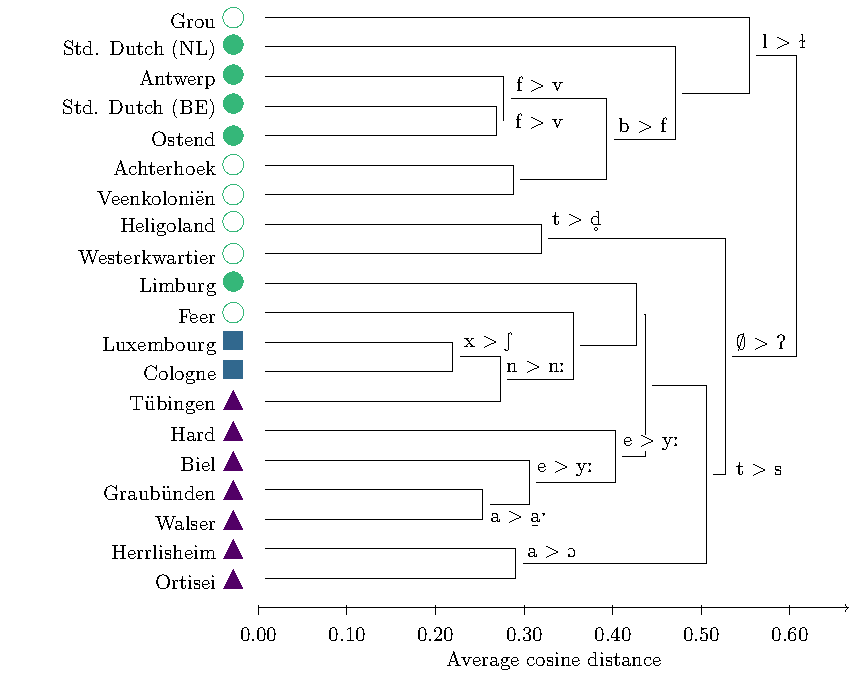
\includegraphics[width=\textwidth]{figures/tfidf-nocontext.pdf}
\end{frame}

\begin{frame}{Appendix}
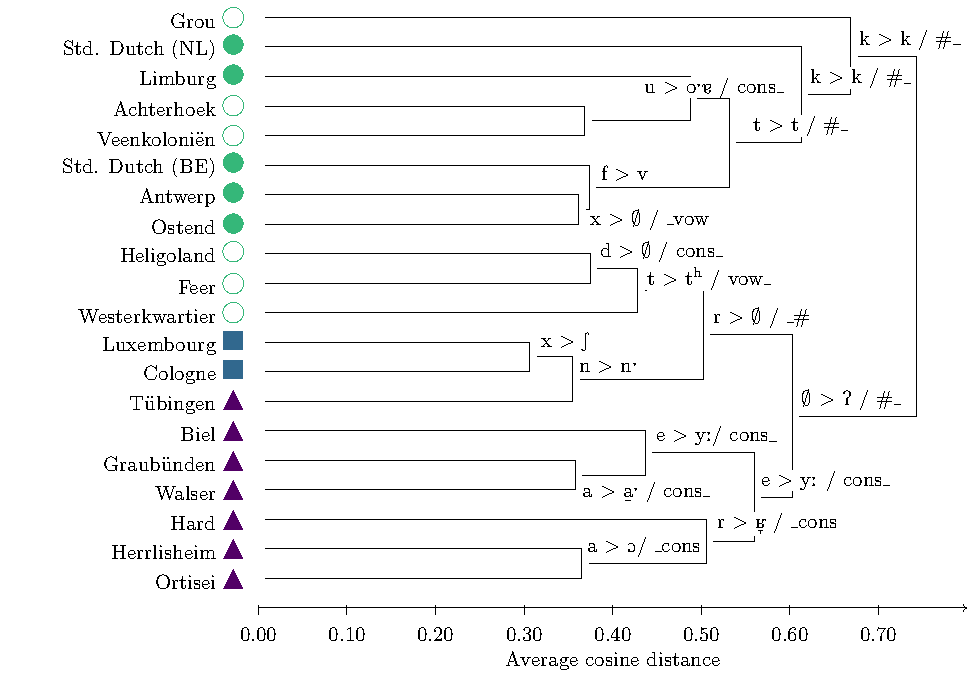
\includegraphics[width=\textwidth]{figures/tfidf-context.pdf}
\end{frame}

\begin{frame}{Appendix}
\begin{figure}[h]
\centering
\includegraphics[width=\textwidth]{figures/bsgc-nocontext.pdf}
\vspace{0.5em}
\begin{center}
\small
{\ingv} Ingv\ae{}onic \hspace{1em}
{\dutch} Dutch \hspace{1em}
{\central} Central German \hspace{1em}
{\upper} Upper German
\end{center}
\end{figure}
\end{frame}

\begin{frame}{Appendix}
\begin{figure}[h]
\centering
\includegraphics[width=\textwidth]{figures/bsgc-context.pdf}\\
\vspace{0.5em}
\begin{center}
\small
{\ingv} Ingv\ae{}onic \hspace{1em}
{\dutch} Dutch \hspace{1em}
{\central} Central German \hspace{1em}
{\upper} Upper German
\end{center}
\end{figure}
\end{frame}

\end{document}
